\documentclass[12pt]{article}
\usepackage[a4paper]{geometry}
\usepackage[utf8]{inputenc}
\usepackage{fancyhdr}
\usepackage{lastpage}
\usepackage{graphicx, wrapfig, subcaption, setspace, booktabs}
\usepackage{graphicx}
\usepackage[T1]{fontenc}
\usepackage[font=small, labelfont=bf]{caption}
\usepackage[protrusion=true, expansion=true]{microtype}
\usepackage[english]{babel}
\usepackage{sectsty}
\usepackage{url, lipsum}
\usepackage[T1]{fontenc}
\usepackage{icomma}
\usepackage{siunitx}
\usepackage{ragged2e}
\usepackage{amsmath}
\usepackage{comment}
\usepackage{enumerate}
\usepackage{anysize}

\newcommand{\HRule}[1]{\rule{\linewidth}{#1}}
\onehalfspacing
\setcounter{tocdepth}{5}
\setcounter{secnumdepth}{5}

\begin{comment}

\end{comment}
\begin{document}

\begin{titlepage}

\title{ \normalsize 
        \begin{center}
        
\includegraphics[height=6cm]{Logo.jpg}
        \end{center}
        \LARGE \textsc{\textbf{Universidad De Sonora}} \\ \bigskip
		\Large División de Ciencias Exactas y Naturales \\
        Licenciatura En Física \\ \bigskip
        \bigskip
        Física Computacional I
		\\ [0.1cm]  
		\HRule{2pt} \\
		\Large \textbf{{Evaluación 2}} \\
        \textit{\textbf{"El Atractor de Lorenz"\\ Ejemplo de Caos Dinámico}}
		\HRule{2pt} \\
		\normalsize \vspace*{0.001\baselineskip}}
        
\date{\bigskip \Large Hermosillo, Sonora  \hspace*{\fill}  Abril 26 de 2018}

        
\author{
		\Large\textbf{ César Omar Ramírez Álvarez} \\ \bigskip
        \\ \bigskip
       \Large Profr. Carlos Lizárraga Celaya}
       \end{titlepage}
       \maketitle
       
\newpage
\pagestyle{plain}
\section*{Introducción}
 El presente reporte constituye parte de la Evaluación número dos de la materia de Física Computacional I, en esta ocasión se utilizó Jupyter Lab como entorno de trabajo, en el que con el uso de sus diversas bibliotecas se da solución a ecuaciones diferenciales para posteriormente realizar su gráfica correspondiente. Analizaremos un ejemplo de caos dinámico como es "El Atractor de Lorenz".\\
 
El sistema de Lorenz es un sistema de ecuaciones diferenciales ordinarias estudiadas por primera vez por Edward Lorenz. Es notable por tener soluciones caóticas para ciertos valores de parámetros y condiciones iniciales. En particular, el atractor de Lorenz es un conjunto de soluciones caóticas del sistema Lorenz que, cuando se trazan, se asemejan a una mariposa o al ocho. En 1963, Edward Lorenz desarrolló un modelo matemático simplificado para la convección atmosférica. En el que las ecuaciones son:\\


\centerline{$\displaystyle \frac{dx}{dt} = \sigma (y-x)$}
\centerline{$\displaystyle \frac{dy}{dt} = x (\rho-z)-y$}
\centerline{$\displaystyle \frac{dx}{dt} = xy-\beta z$}
$ $\\
Las ecuaciones relacionan las propiedades de una capa de fluido bidimensional uniformemente calentada desde abajo y enfriada desde arriba. En particular, las ecuaciones describen la tasa de cambio de tres cantidades con respecto al tiempo: $x$ es proporcional a la velocidad de convección, $y$ a la variación de temperatura horizontal, y  $z$ a la variación de temperatura vertical. Las constantes $\sigma$ , $\rho$ y $\beta$ son parámetros del sistema proporcionales al número de Prandtl , número de Rayleigh y ciertas dimensiones físicas de la capa misma.\\

Con el apoyo de un segmento de código tomado desde un blog de Geoff Boeing se realizó un análisis para distintos valores de $\sigma$, $\rho$ y $\beta$ creando también la representación gráfica correspondiente, a continuación el análisis de los resultados.

\section*{Análisis de Resultados}
Con el apoyo del segmento de código ya proporcionado, trabajaremos en Jupyter Lab para resolver 3 casos en los que cambian los valores de $\sigma$, $\rho$ y $\beta$ crearemos gráficas y un gif (se visualizará en el archivo .ipynb) con los resultados arrojados.

\subsection*{Ejercicio 1}
Para este caso, los valores son $\sigma= 10$, $\rho=28$ y $\beta=\frac{8}{3}$\\
La gráfica de fase en 3D obtenida es:
\begin{center}
    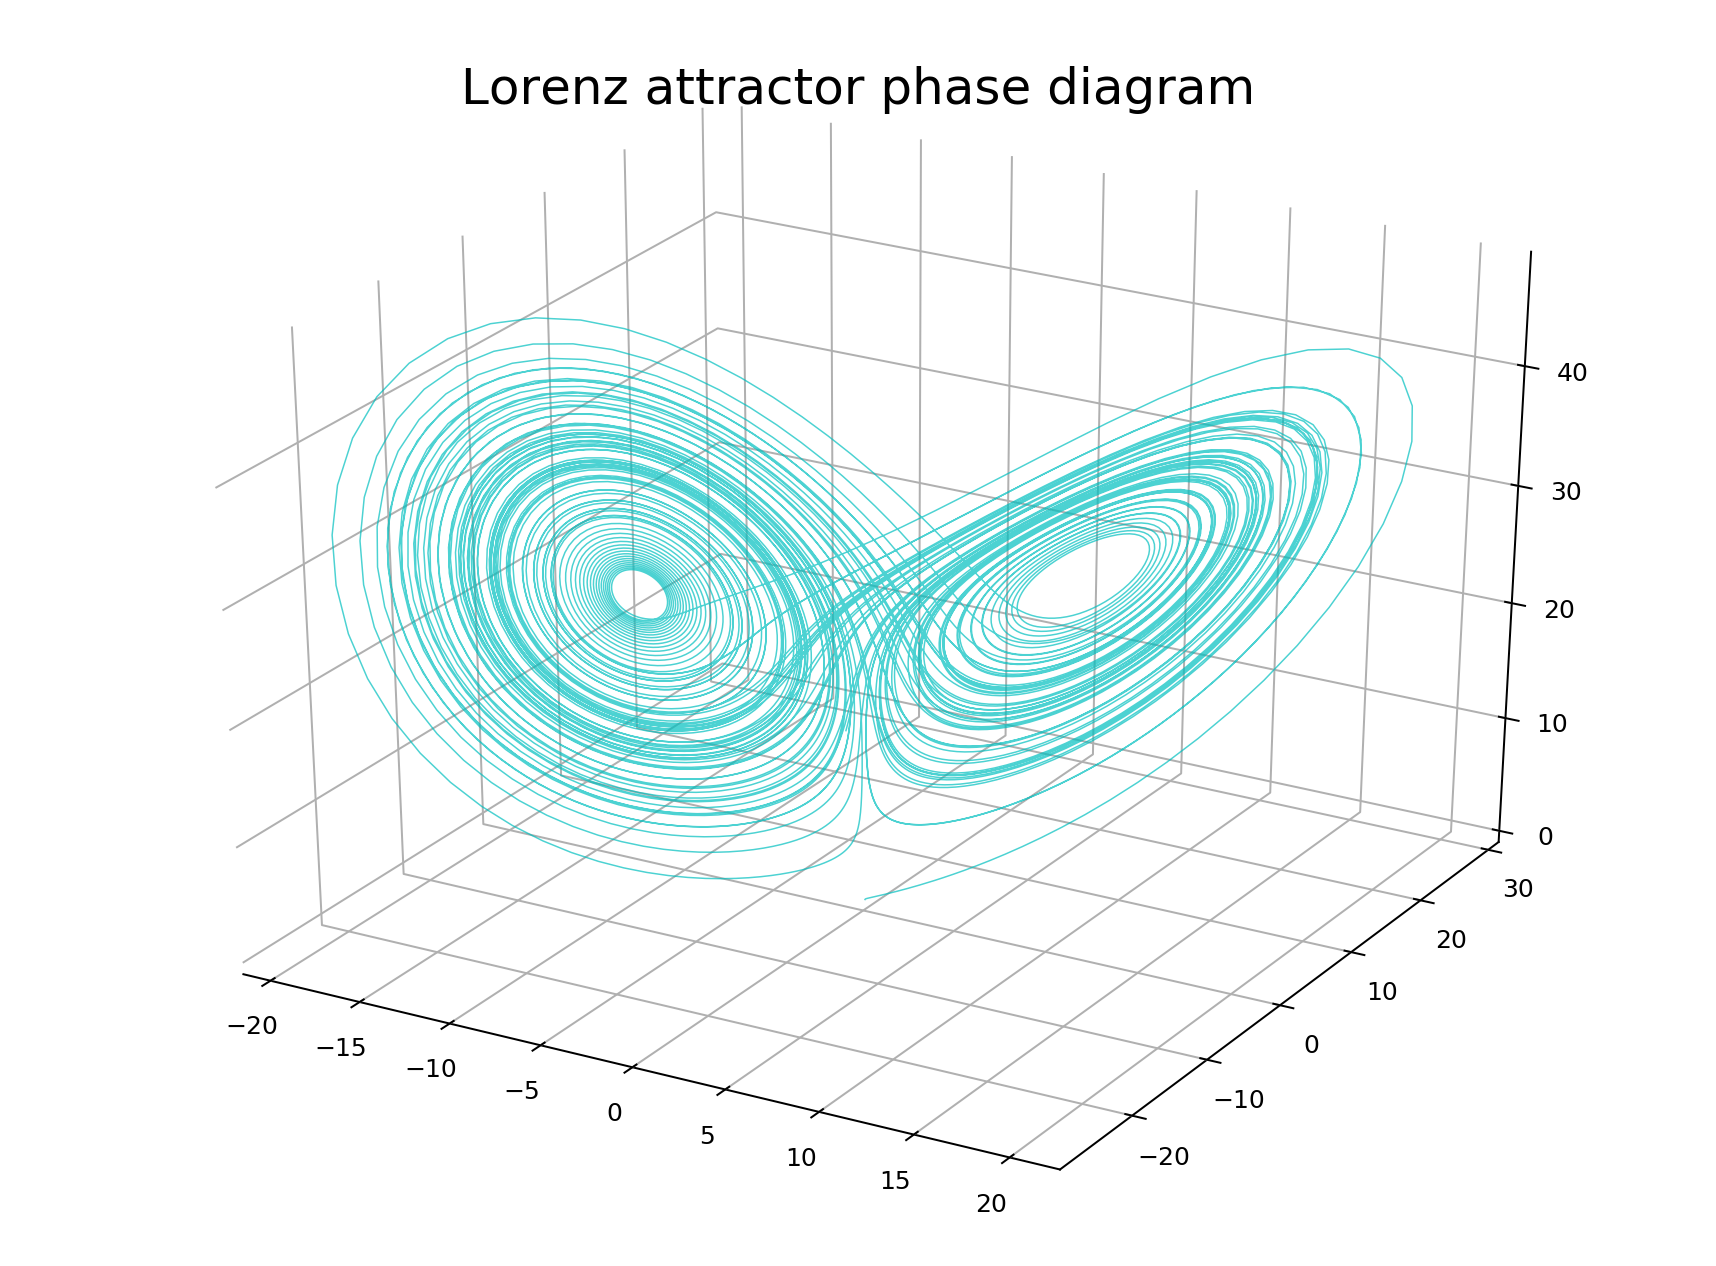
\includegraphics[height=9cm]{lorenz-attractor-3d1.png}\\
\end{center}
Podemos describir la gráfica asemejandola a un ocho, o bien a las alas de una mariposa. Mostrando como el caos se ata a ciertos parámetros.\\

La gráfica de retrato de fase para cada uno de los planos es:
\begin{center}
    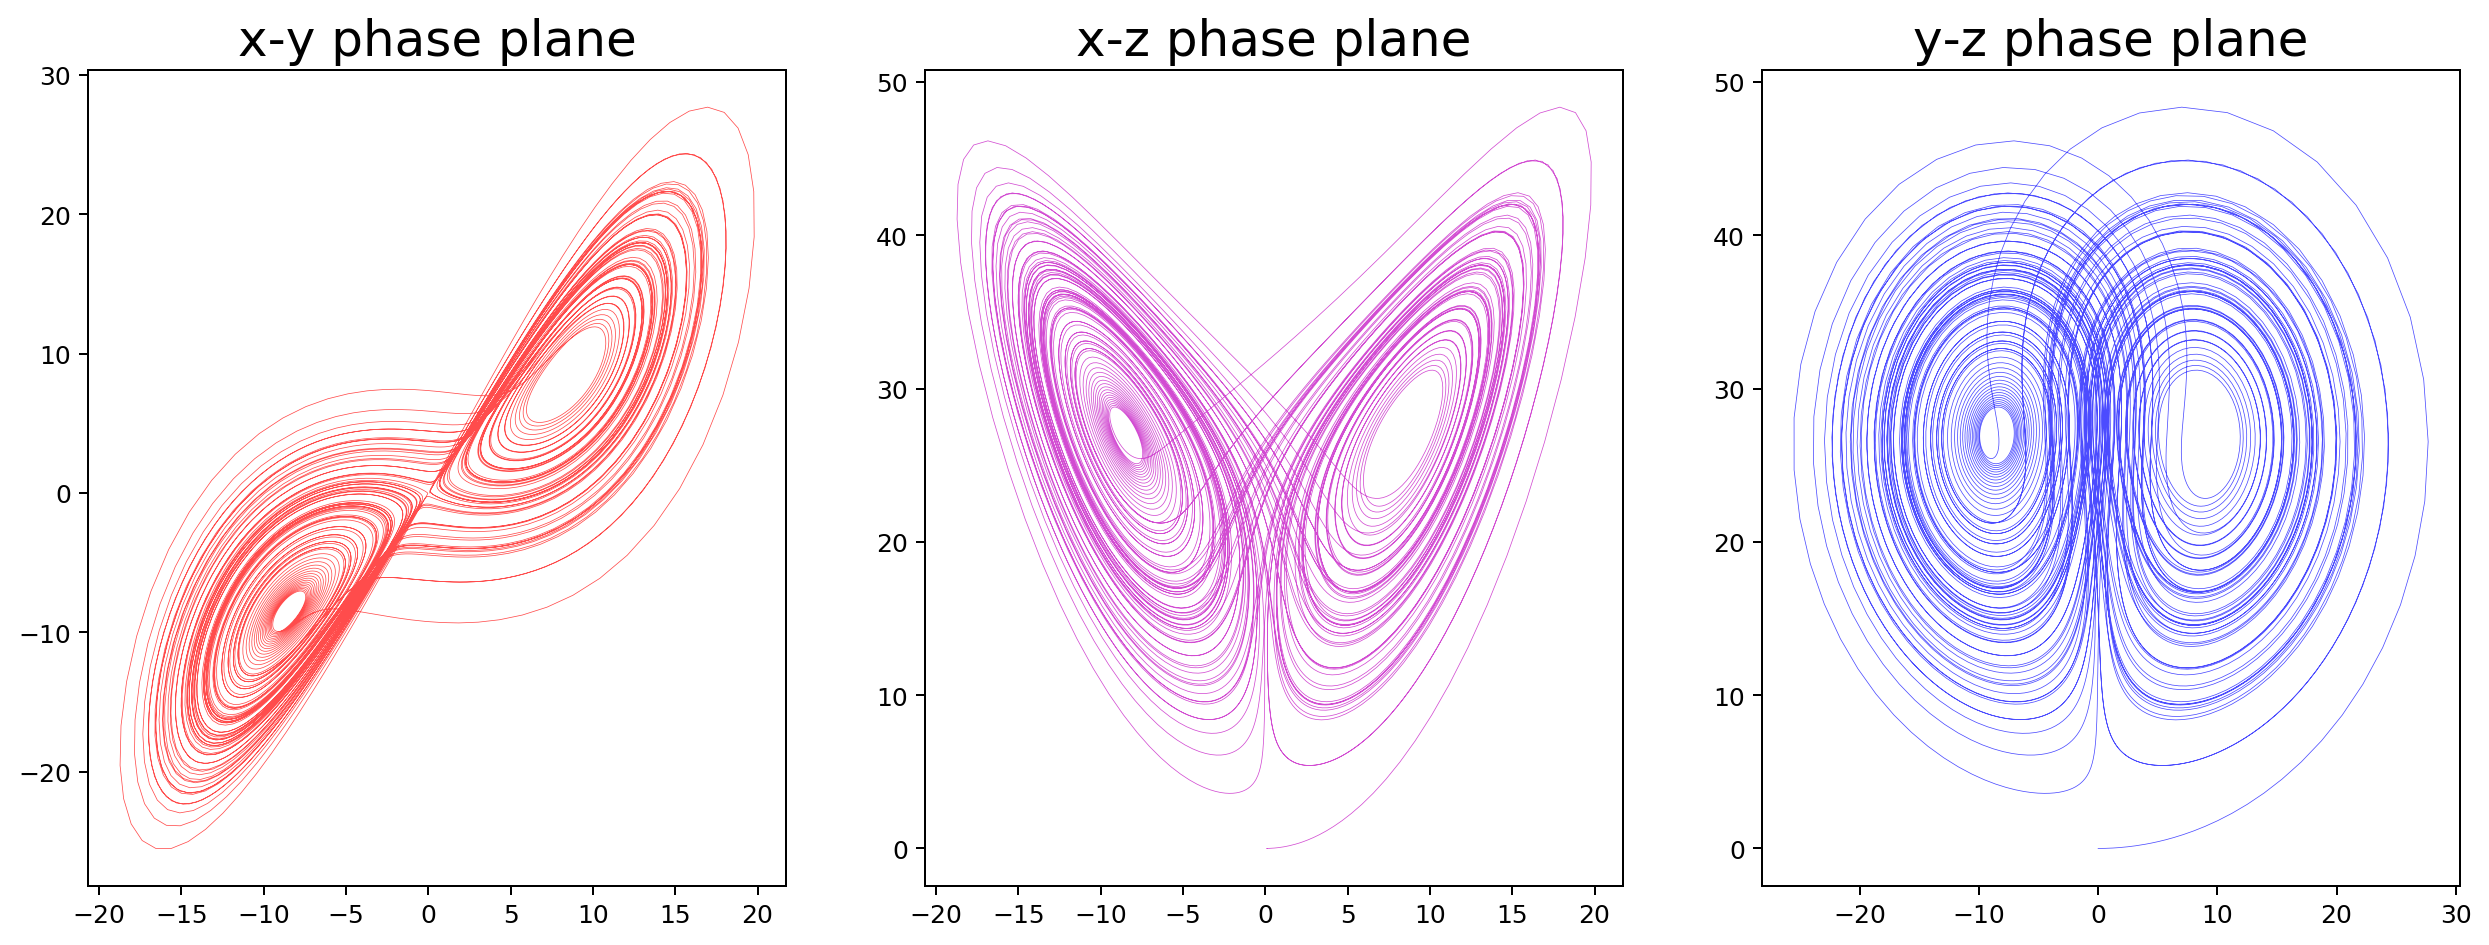
\includegraphics[height=6cm]{lorenz-attractor-phase-plane1.png}\\
\end{center}
Notamos que para cada plano no es la misma percepción de la forma que tienen, ya que para el plano $xy$ asemeja mas a un ocho y mientras para $xz$ y $yz$ se asemejan a las alas de una mariposa.\\

La gráfica de la posición en el tiempo para cada una de las variables $x, y$ y $z$ es:
\begin{center}
    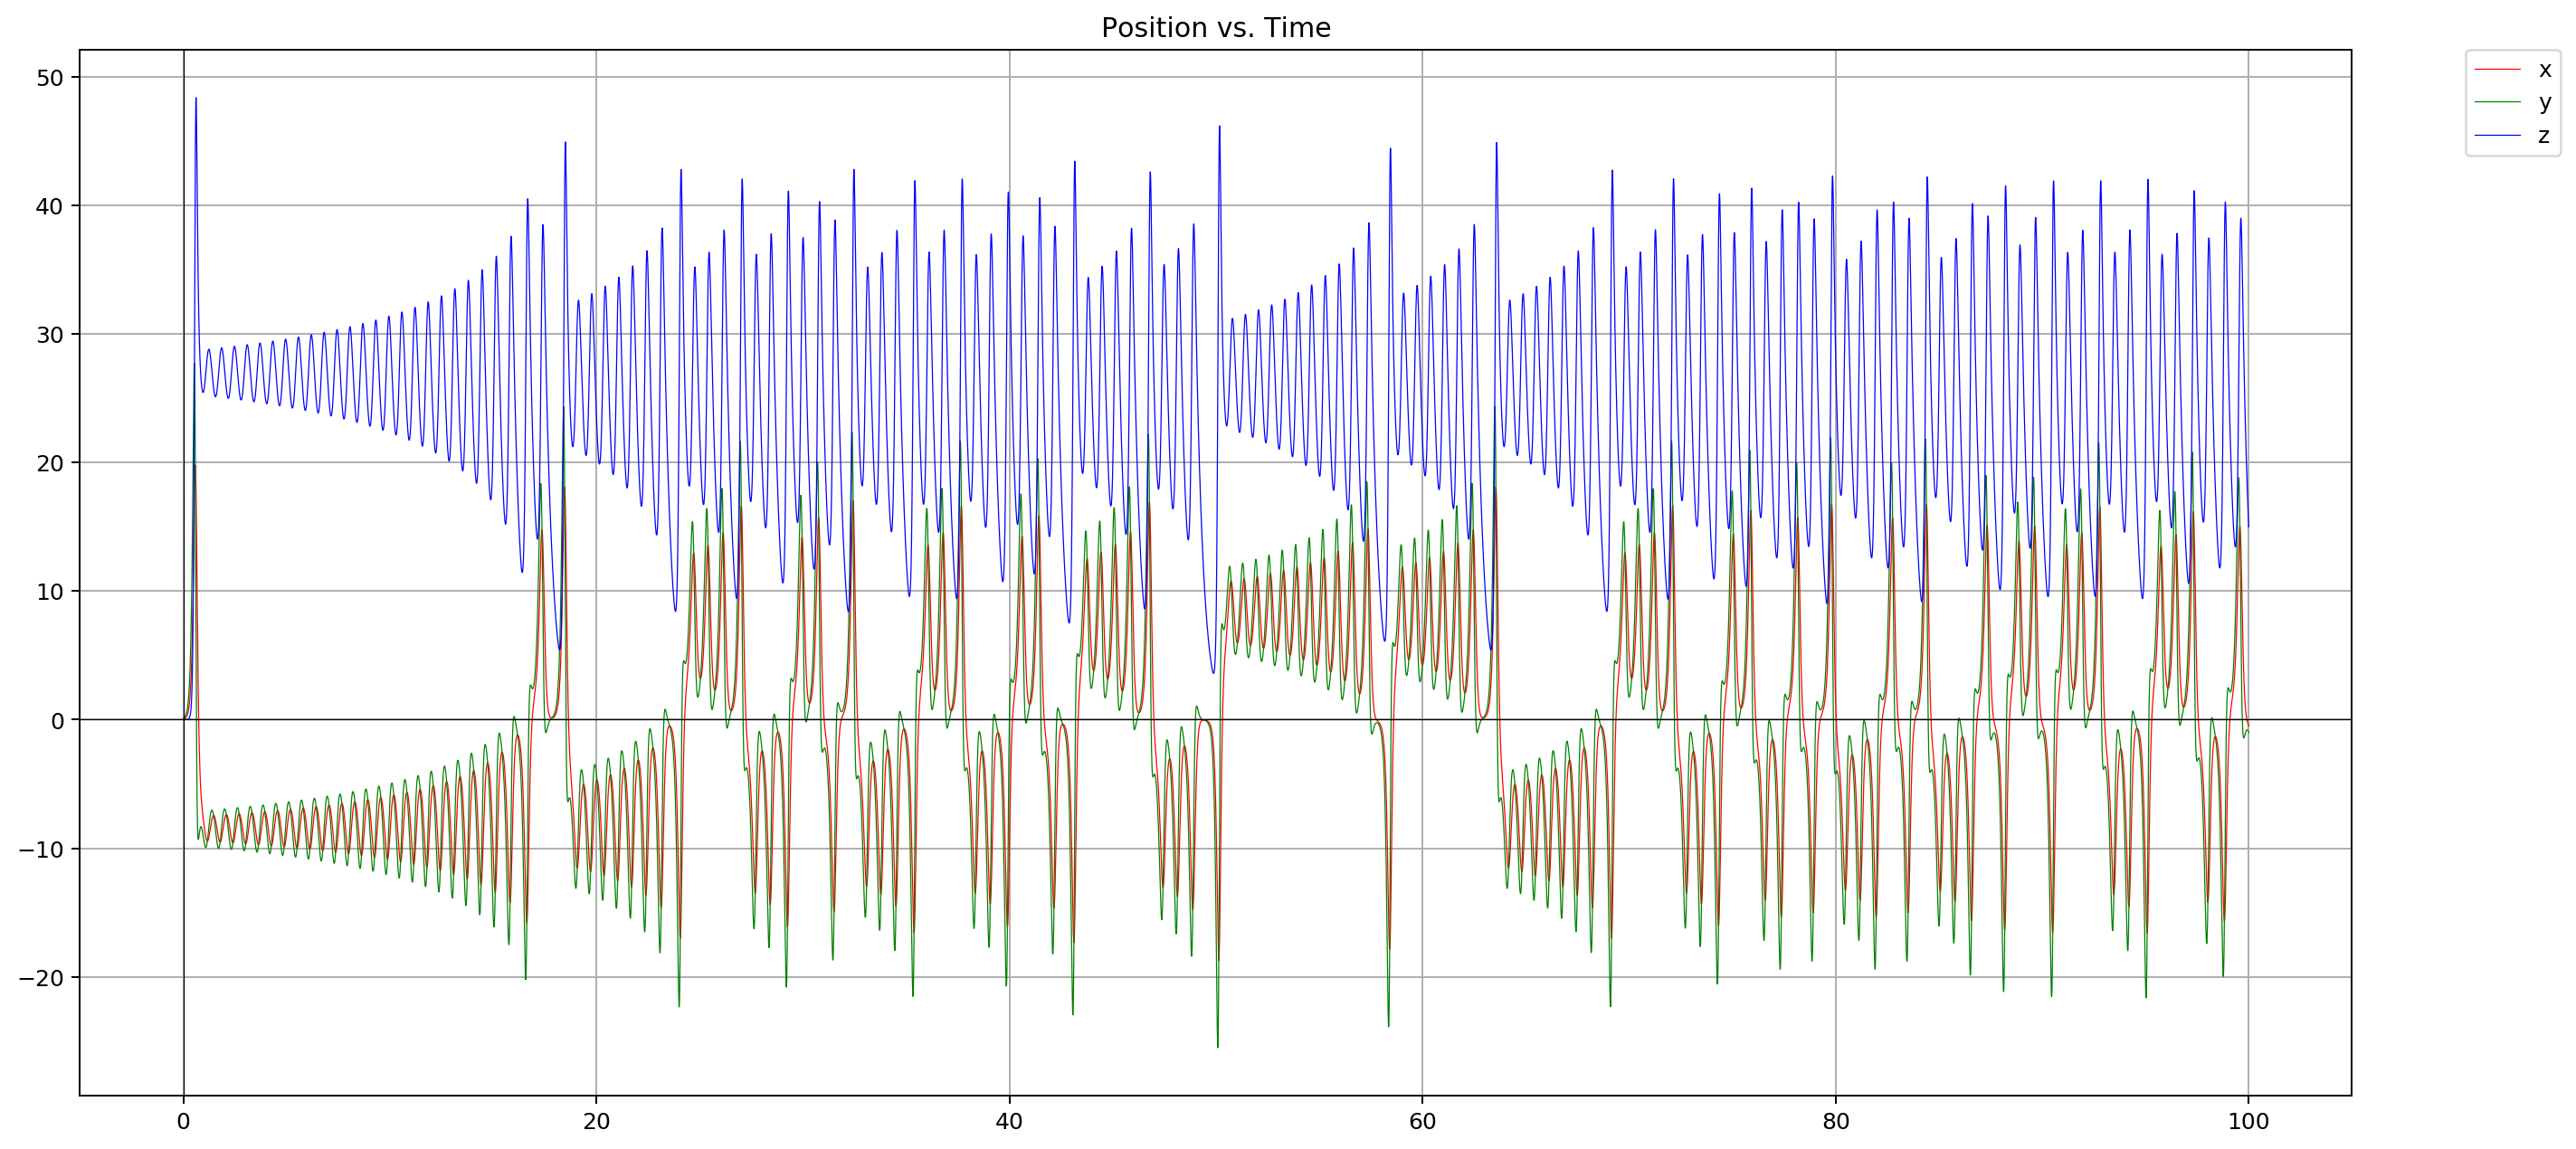
\includegraphics[height=7cm]{AtractorLorentzPosicion1.png}\\
\end{center}
De ésta gráfica es rescatable que $z$ oscila solo por arriba de 0, mientras que $x$ y $y$ tienen comportamiento parecido y si cruzan el 0. Como es caótico no se repite una misma trayectoria por la que ya hayan atravesado alguna vez.

\subsection*{Ejercicio 2}
Para este caso, los valores son $\sigma= 28$, $\rho=46.92$ y $\beta=4$\\
La gráfica de fase en 3D obtenida es:
\begin{center}
    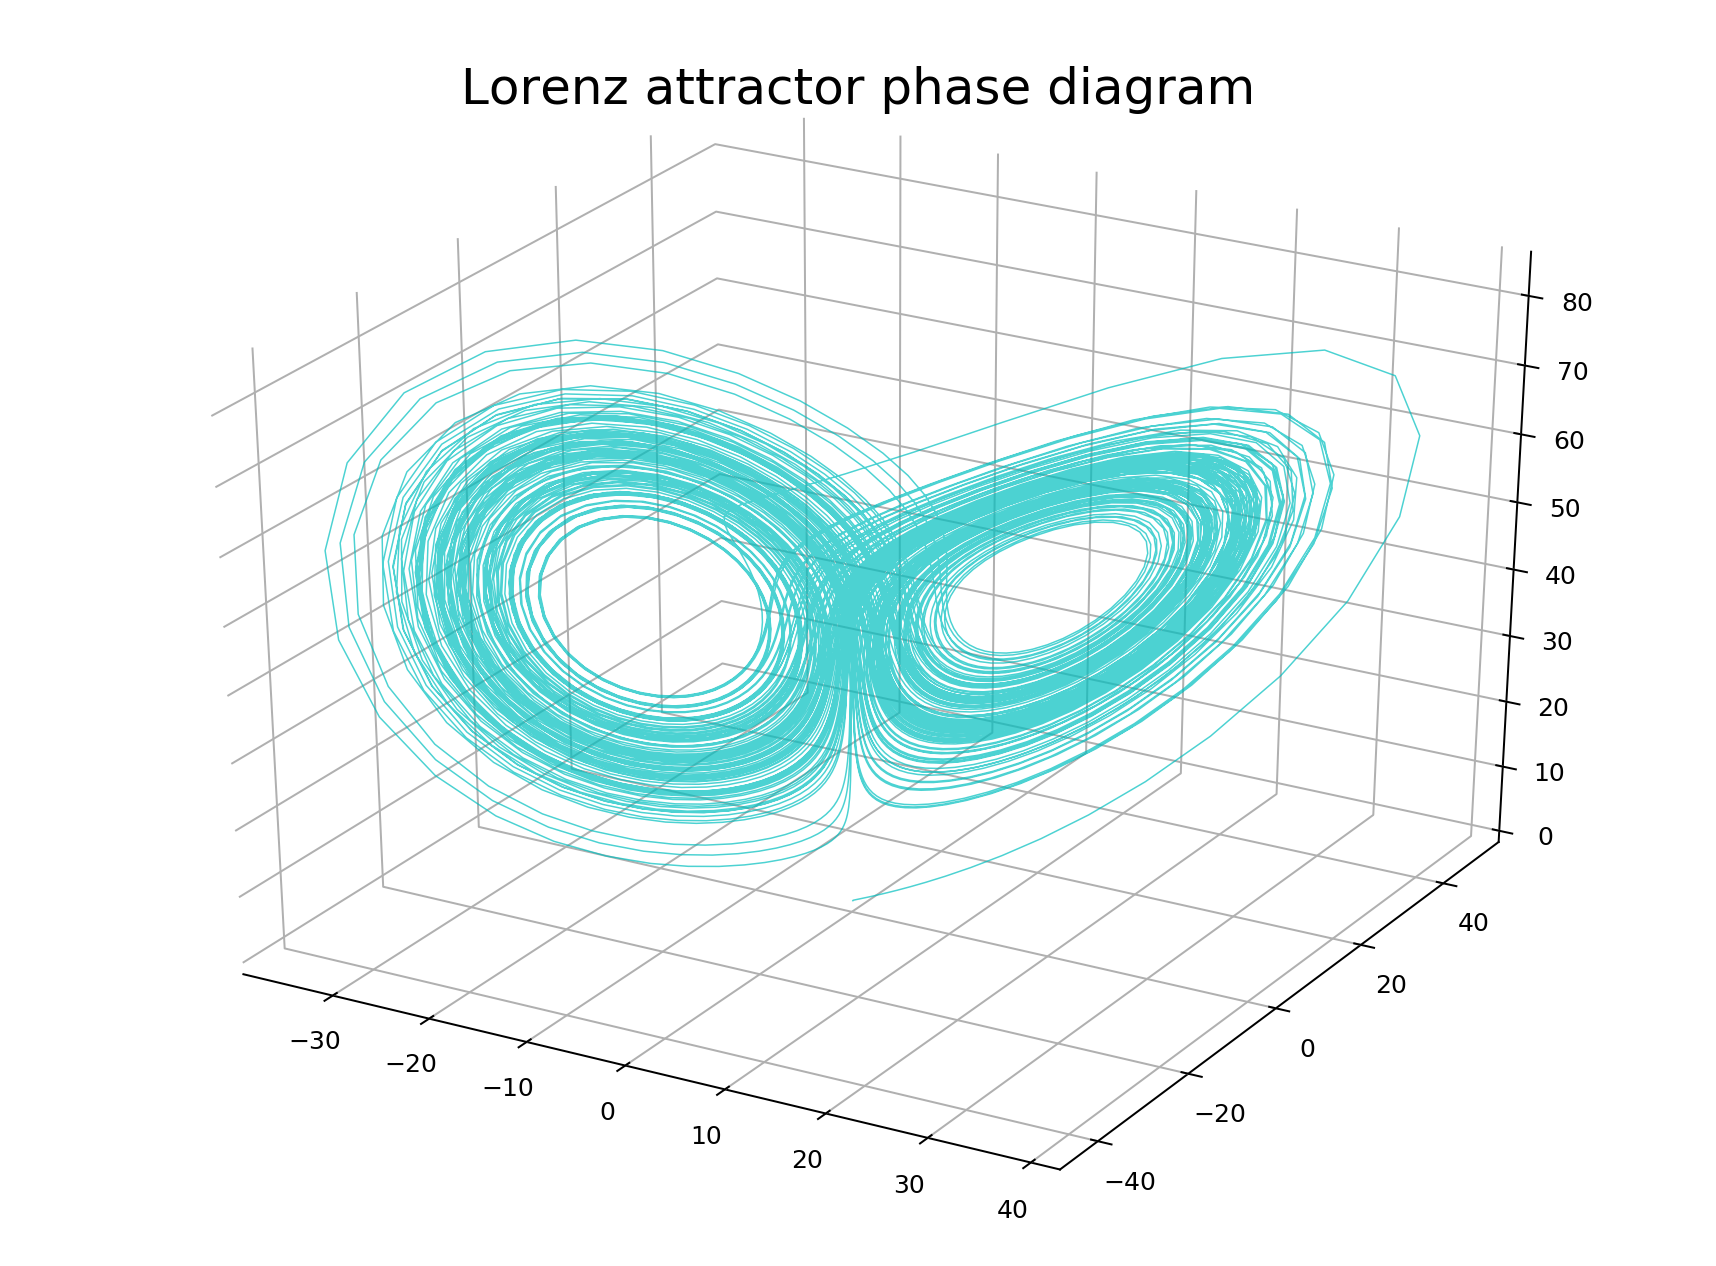
\includegraphics[height=9cm]{lorenz-attractor-3d2.png}\\
\end{center}
Este caso se muestra muy parecido al anterior, solo que aquí el "ocho" ya no es tan relleno y esta mas bien figurado (sus perforaciones).\\

La gráfica de retrato de fase para cada uno de los planos es:
\begin{center}
    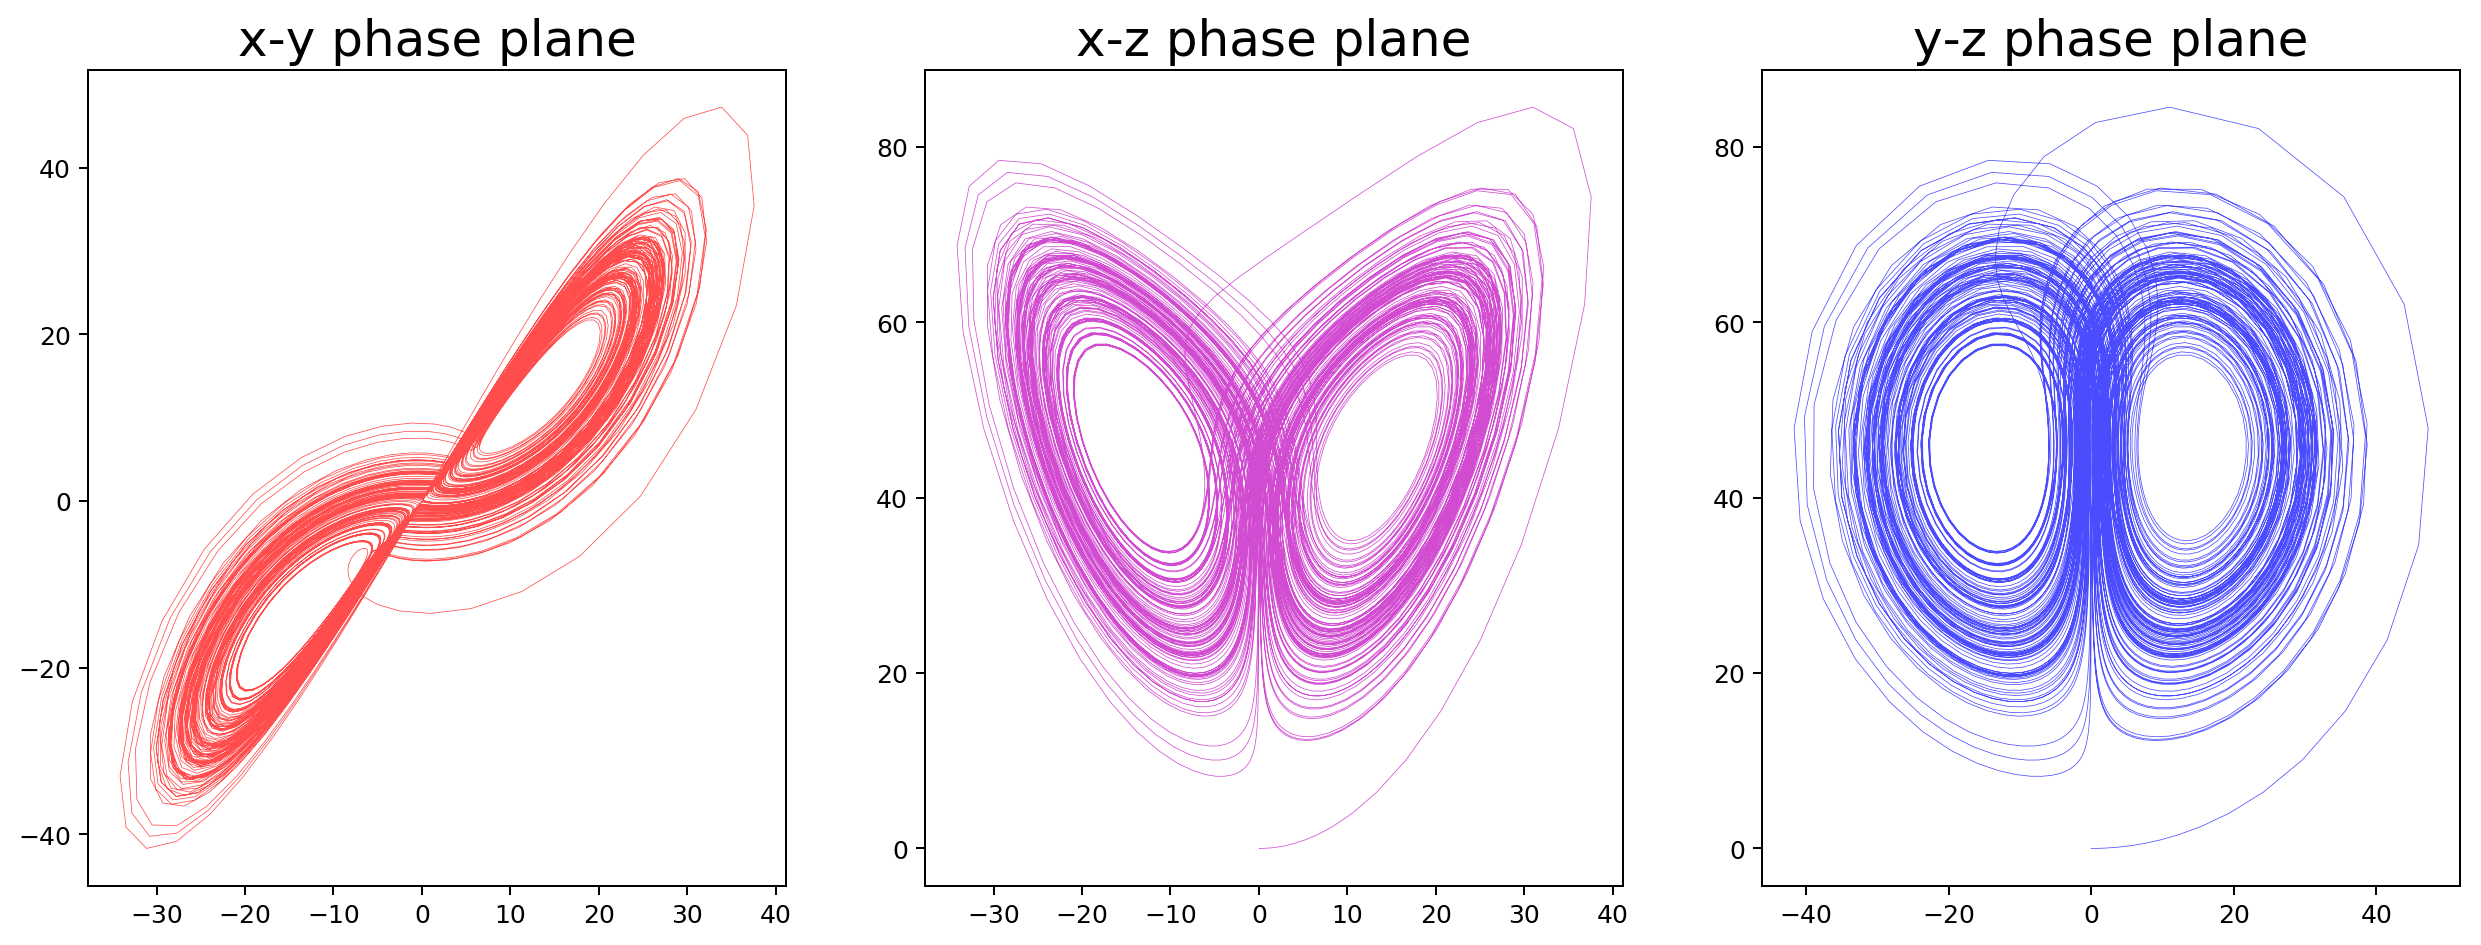
\includegraphics[height=6cm]{lorenz-attractor-phase-plane2.png}\\
\end{center}
Notamos la similitud con el caso anterior, resaltando que ahora son mas notorias las perforaciones.\\

La gráfica de la posición en el tiempo para cada una de las variables $x, y$ y $z$ es:
\begin{center}
    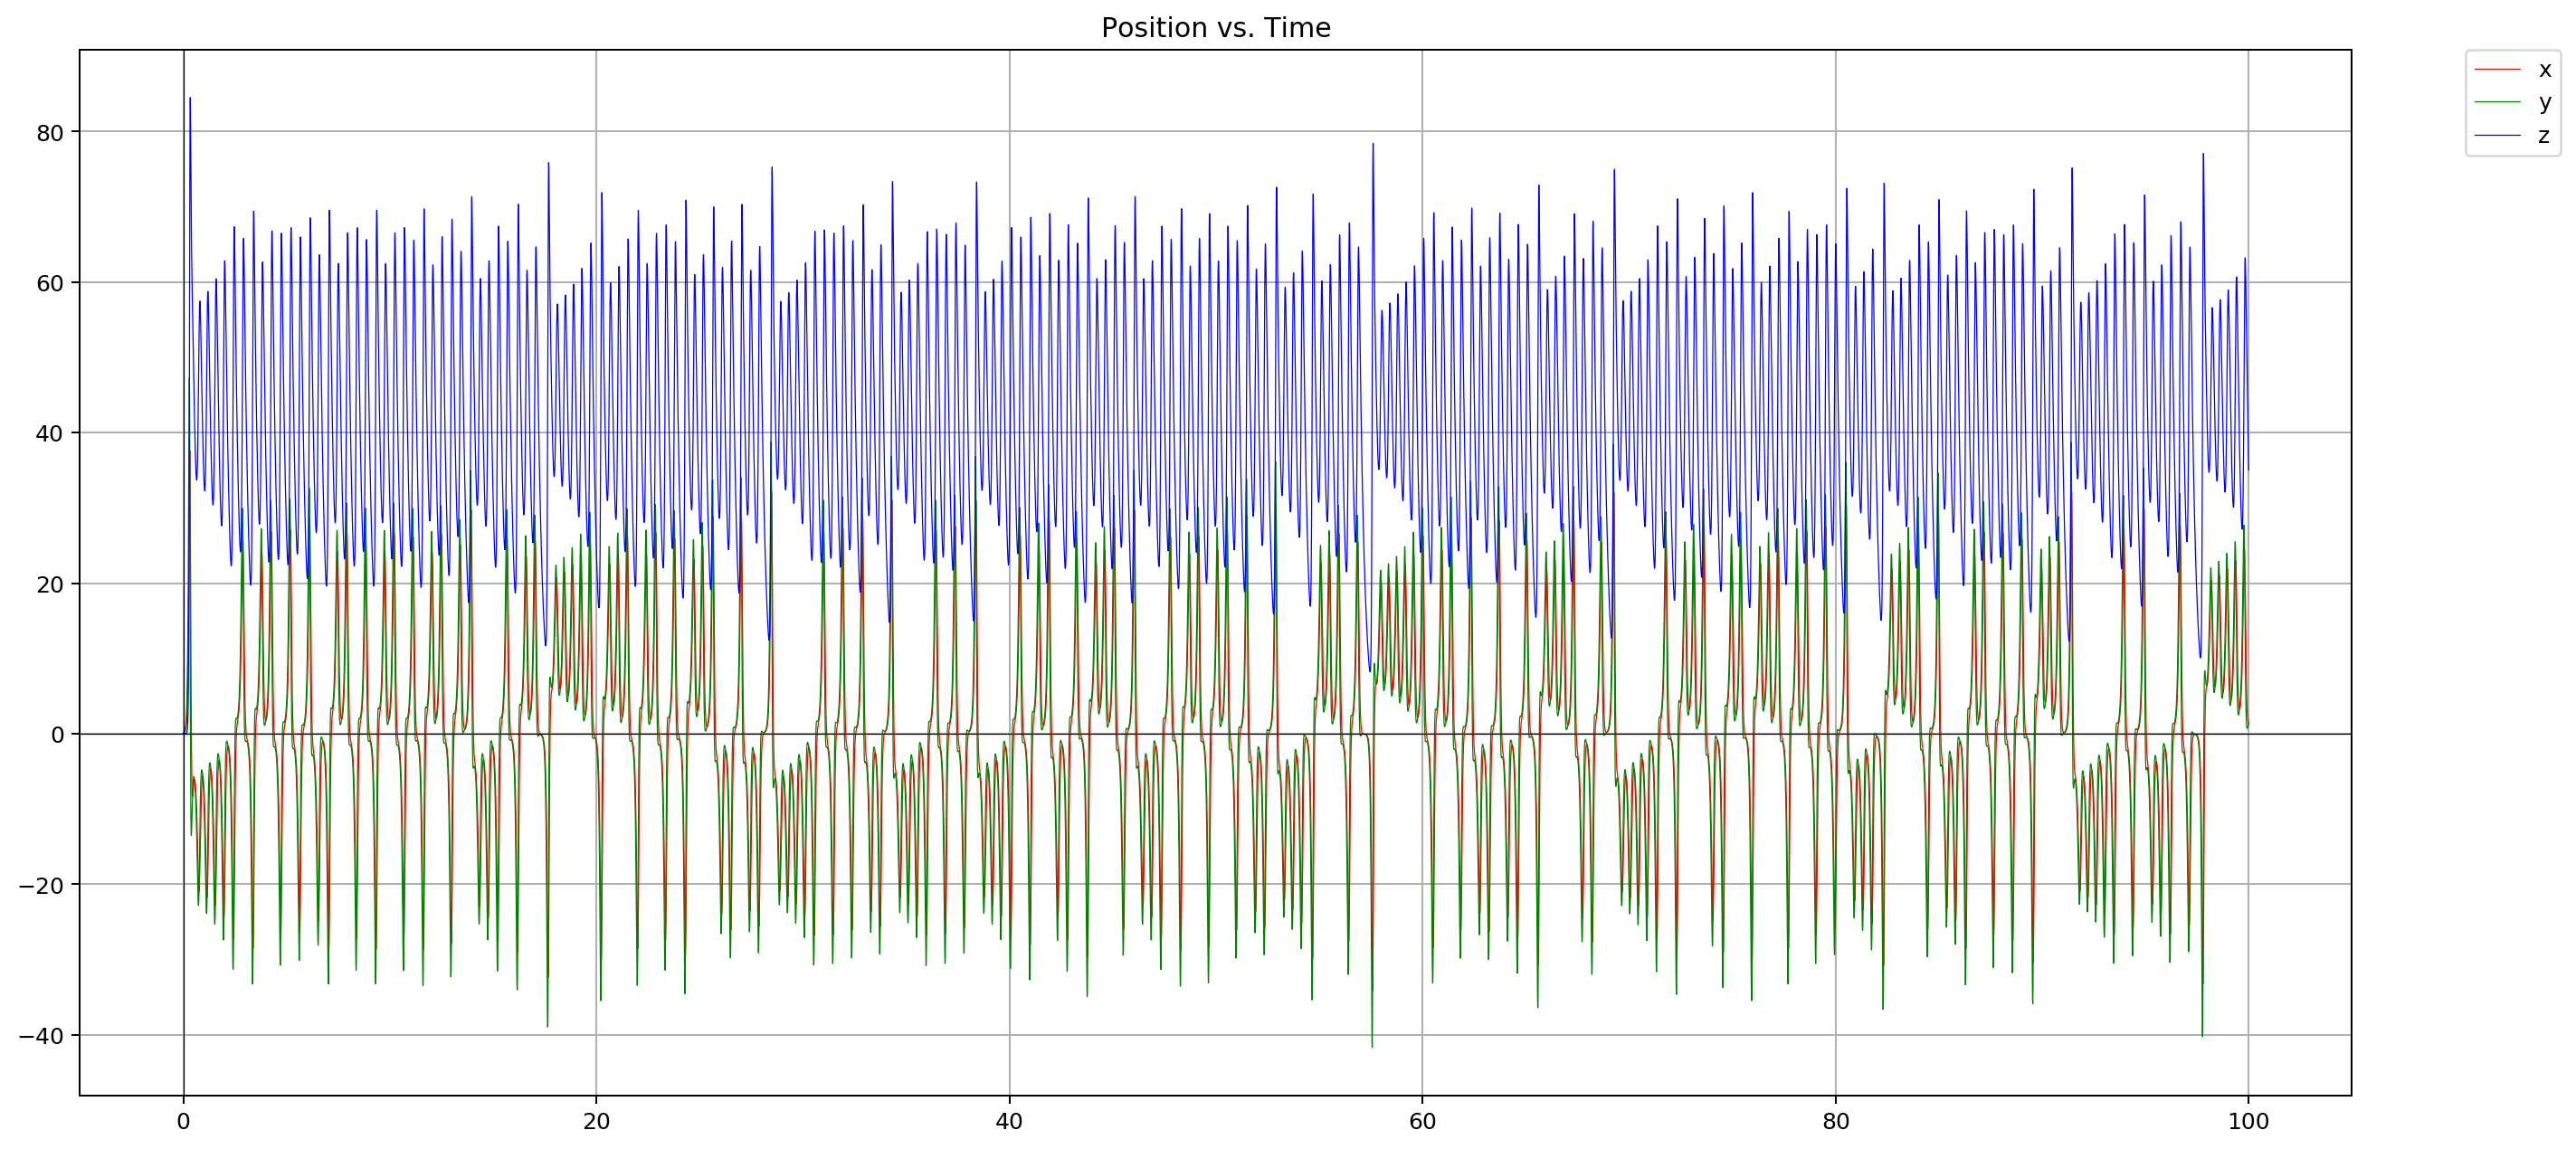
\includegraphics[height=7cm]{AtractorLorentzPosicion2.png}\\
\end{center}
Con esta gráfica son mas notorias las similitudes entre los ejemplos 1 y 2, ya que la $z$ se sigue comportando por arriba del 0 y mientras que $x$ y $y$ suelen parecerse pero ahora con presencia de mas caos.

\subsection*{Ejercicio 3}
Para este caso, los valores son $\sigma= 10$, $\rho=99.96$ y $\beta=\frac{8}{3}$\\
La gráfica de fase en 3D obtenida es:
\begin{center}
    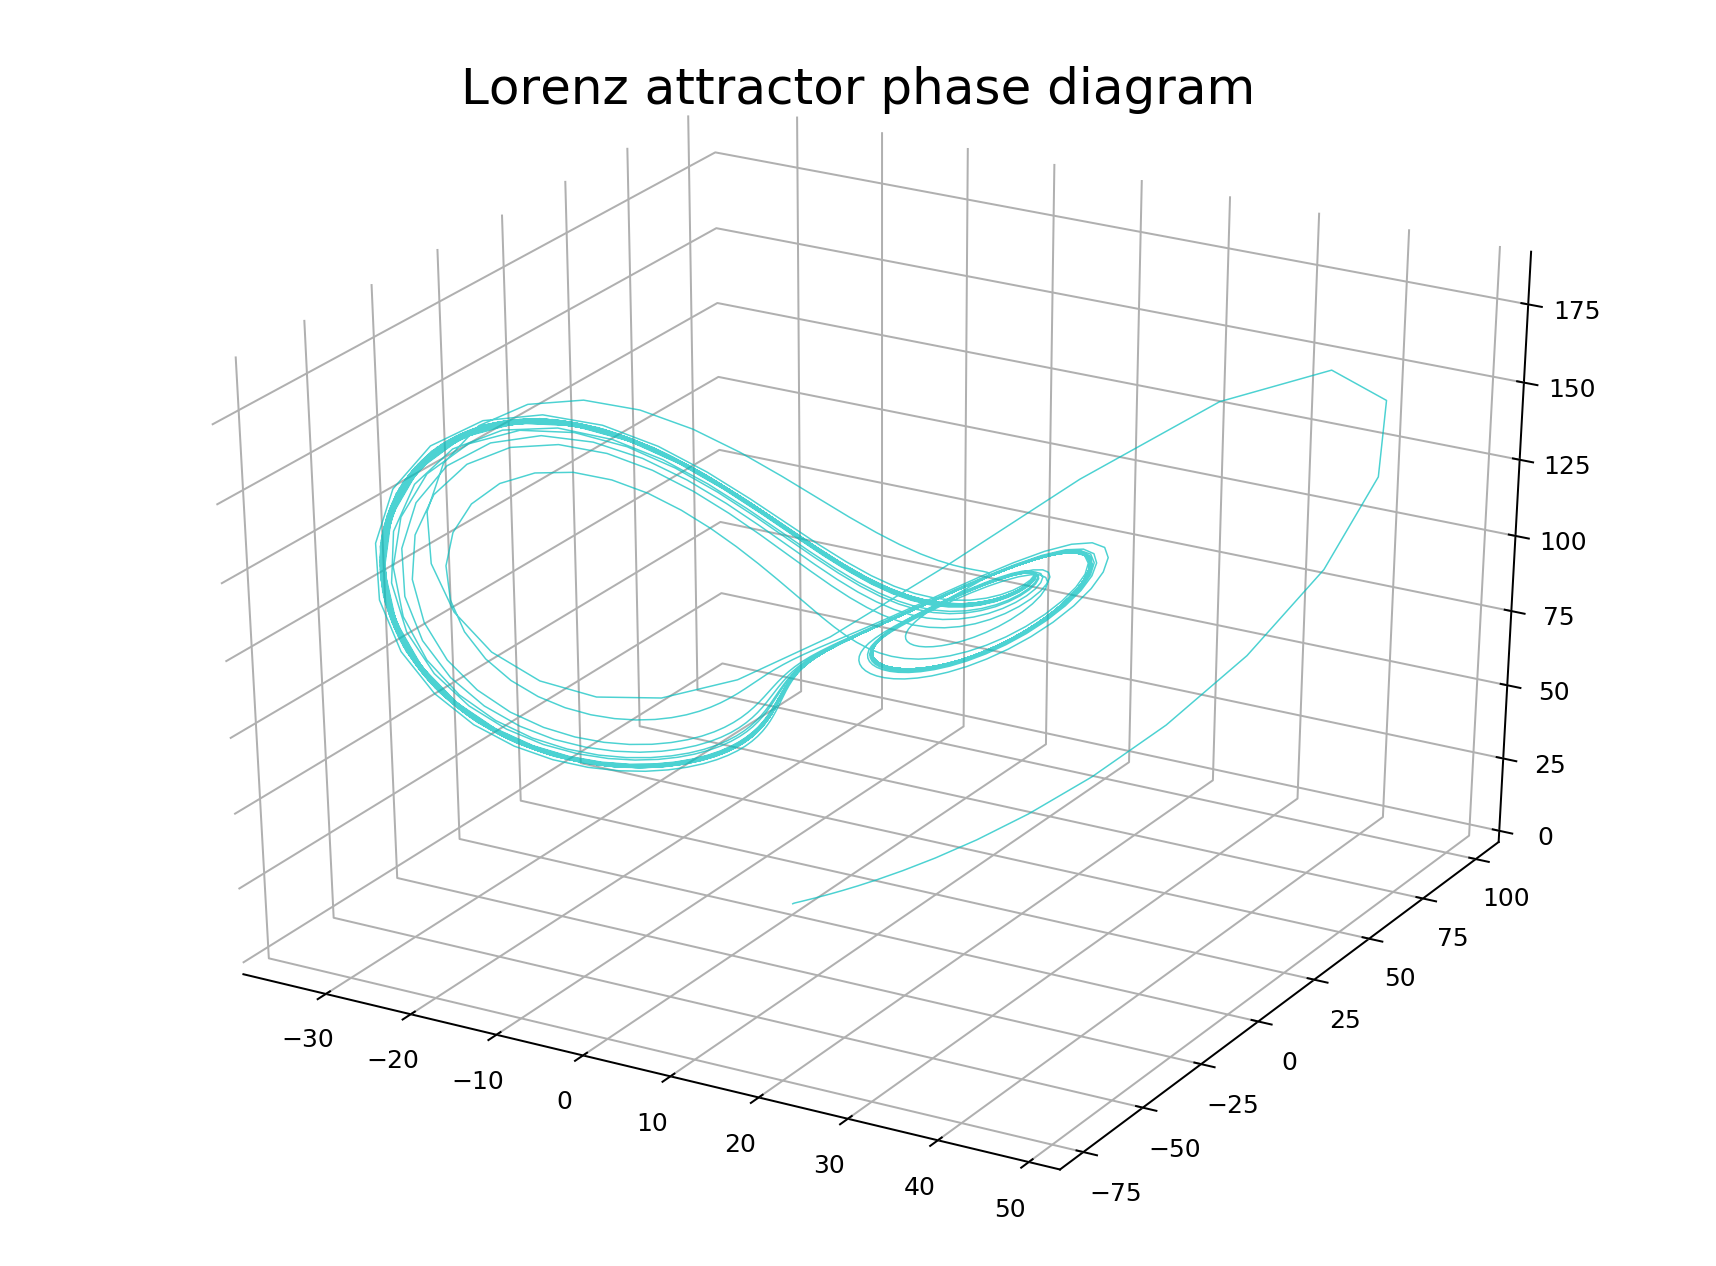
\includegraphics[height=9cm]{lorenz-attractor-3d3.png}\\
\end{center}
Ahora nos encontramos con un caso el cual no sigue tanto un patron como los anteriores, si no que vemos que aun así se inclina mas por el eje negativo de las $x$, por otro lado al notar que los datos son iguales que en el ejercicio 1, excepto por el parámetro $\rho$ lo cual nos pudiera decir que mientras mas significativo el cambio en uno de los parámetros mas caos se observa.\\

La gráfica de retrato de fase para cada uno de los planos es:
\begin{center}
    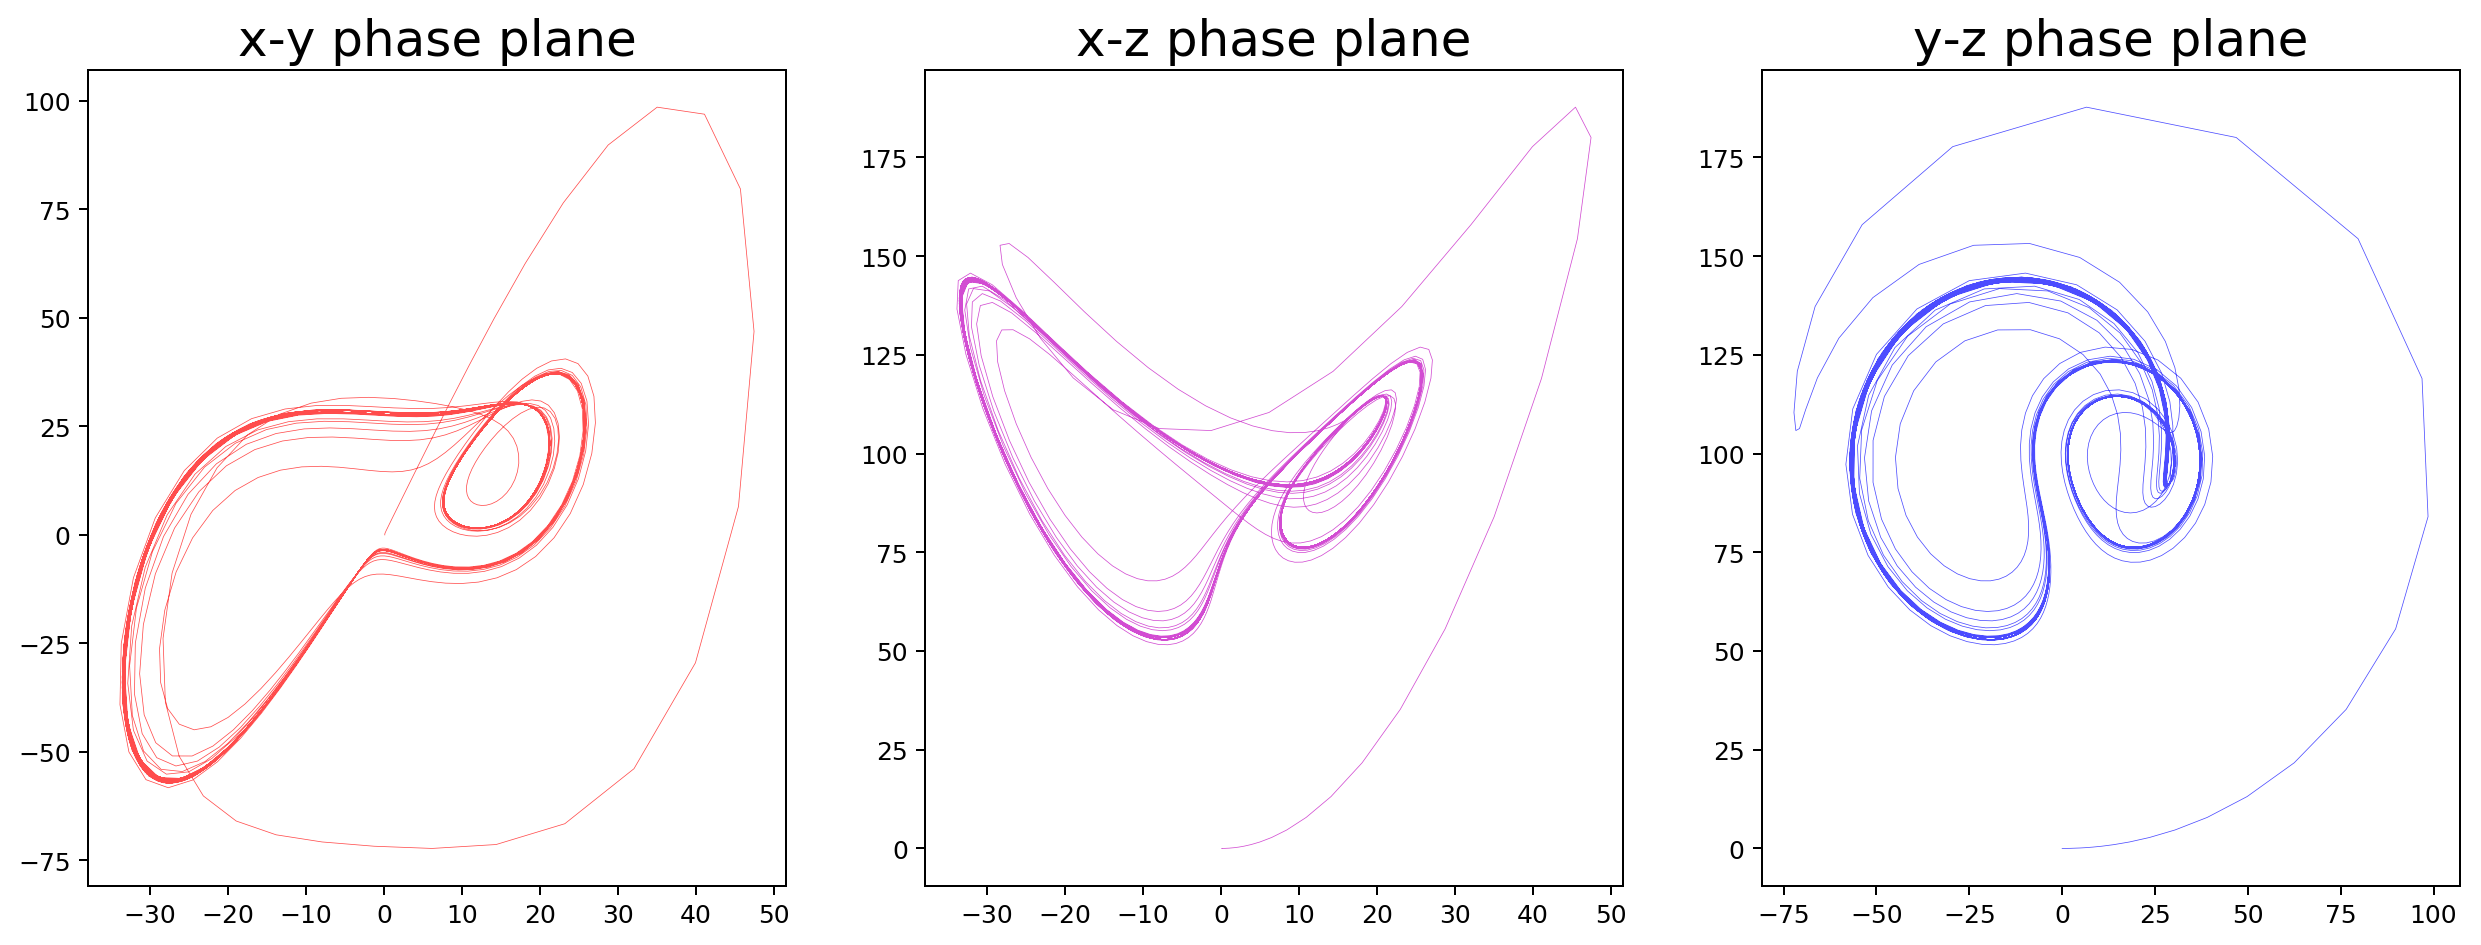
\includegraphics[height=6cm]{lorenz-attractor-phase-plane3.png}\\
\end{center}
No se nota que ninguna figura los relacione, por lo que se concluye que es un sistema muy caótico.\\

La gráfica de la posición en el tiempo para cada una de las variables $x, y$ y $z$ es:
\begin{center}
    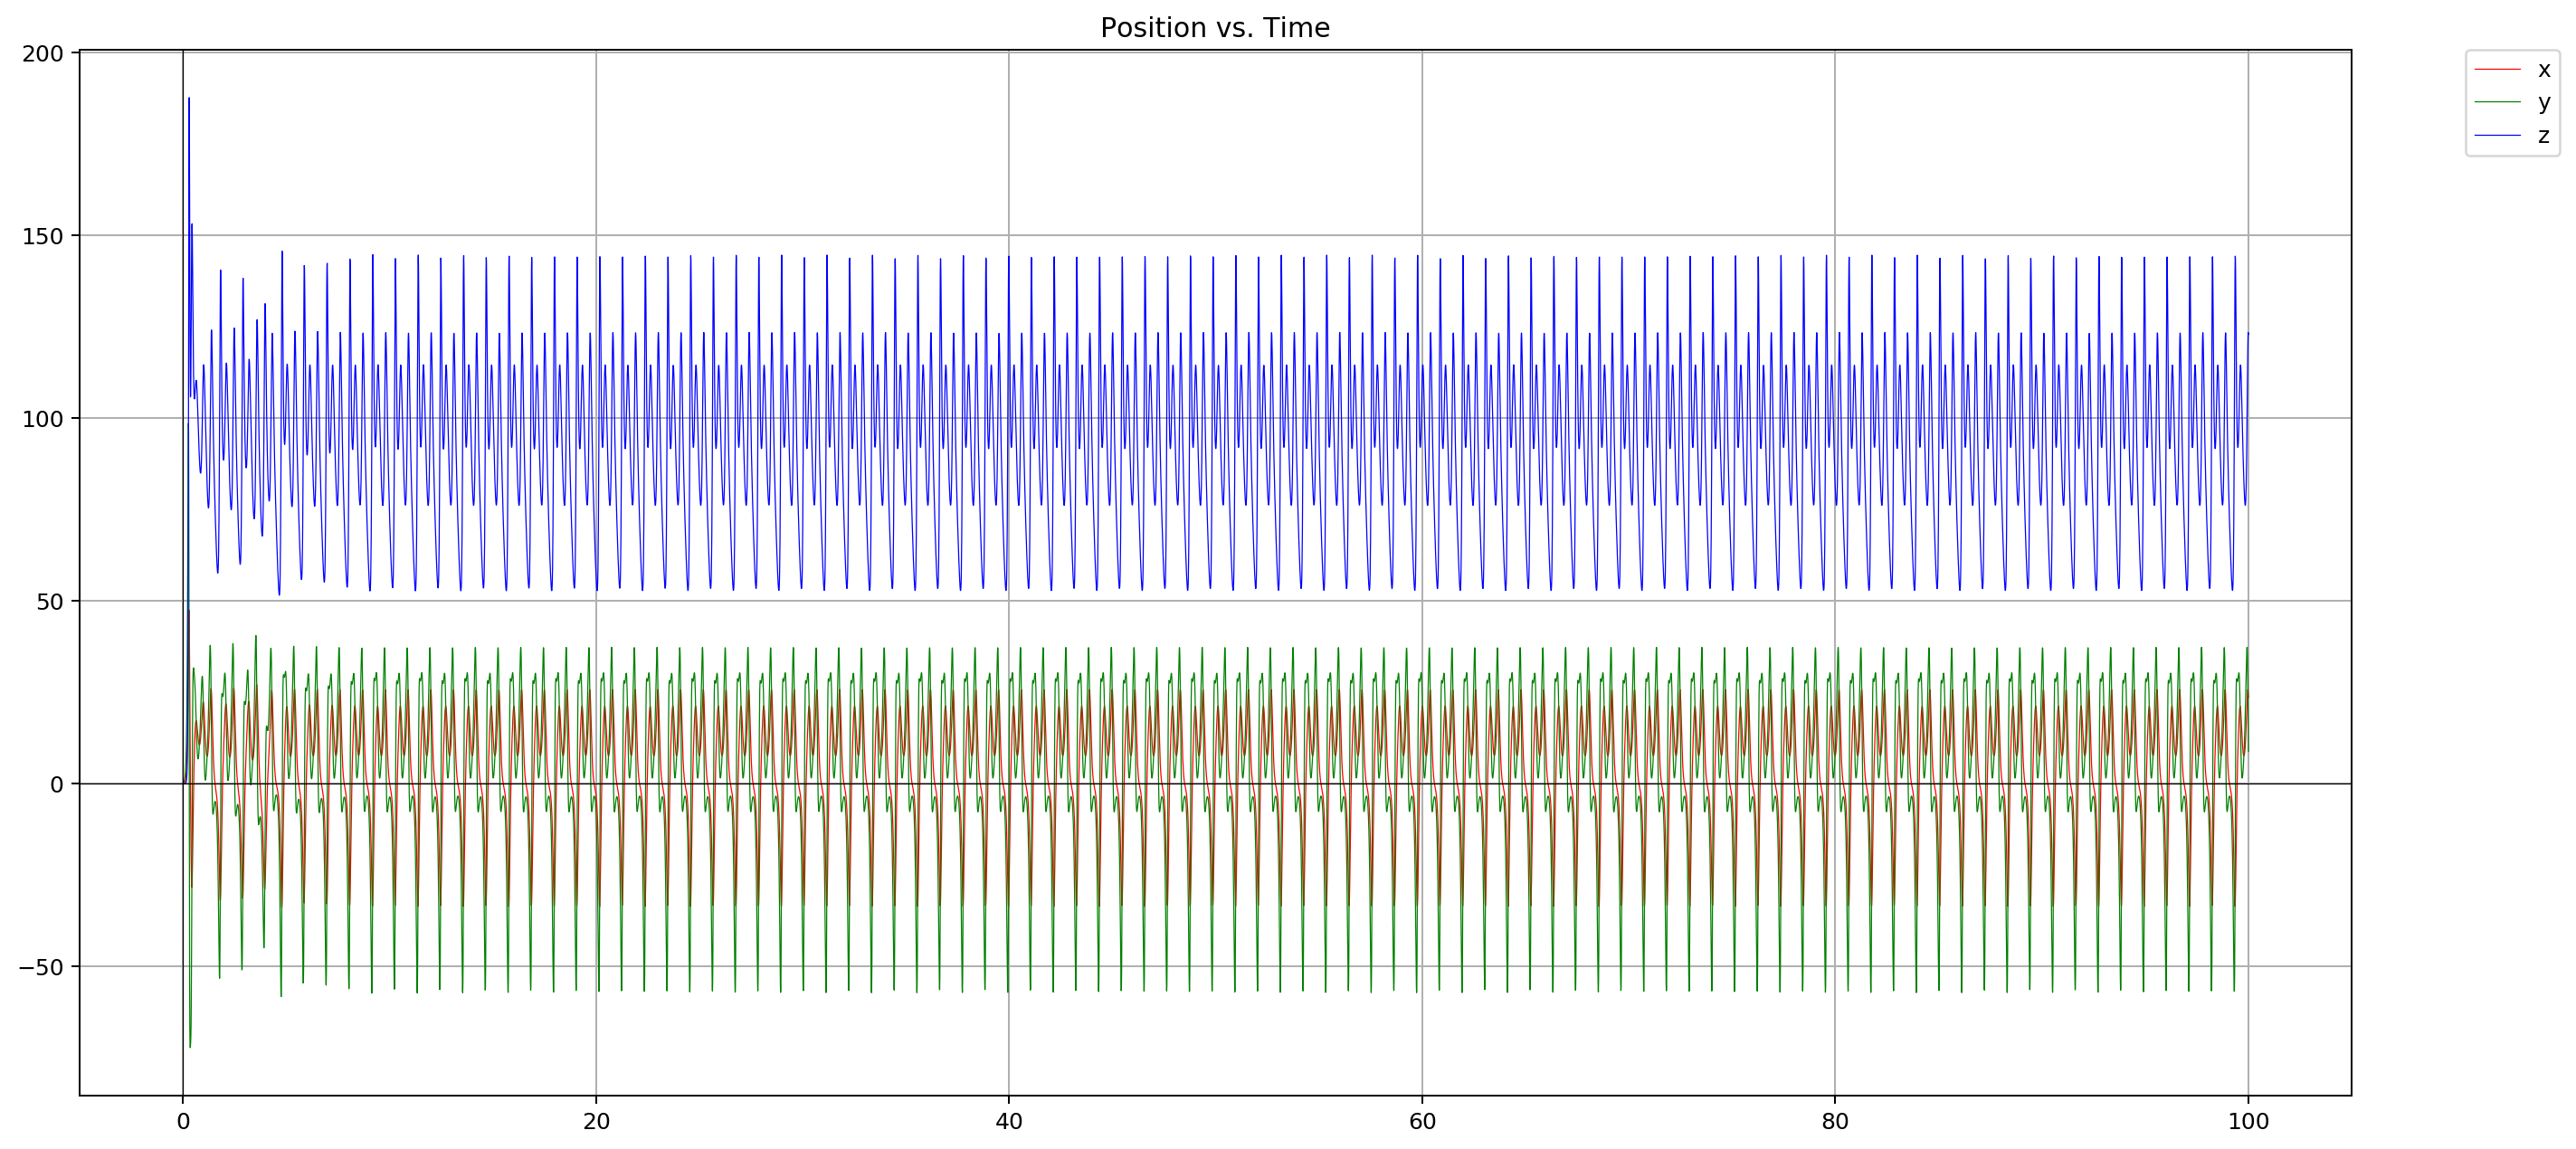
\includegraphics[height=7cm]{AtractorLorentzPosicion3.png}\\
\end{center}
Es notorio que $z$ se sigue comportando de la misma manera que en los anteriores, mientras que $x$ y $y$ se representan de una manera más caótica por sus trayectorias.

\section*{Conclusión}
Con todas las actividades realizadas hasta hoy y como complemento esta evaluación nos hace darnos cuenta de los pros que tenemos al utilizar el lenguaje Python y todas sus bibliotecas para la resolución de problemas, tanto ver la forma numérica como la parte de graficación en 2D y 3D.\\

Con un poco de destiempo, pero me fué posible completar esta actividad de evaluación, incluyendo los "gif's" producidos y las demás gráficas. Además de que la ejemplificación del tema con el "Atractor de Lorenz" me pareció muy interesante y el hecho de introducir graficación 3D hace razonar mas el análisis de las situaciones que se presentan.

\section*{Bibliografía}
\begin{itemize}
\item gboeing/lorenz-system. (2018). GitHub. Recuperado el 26 Abril 2018, desde\\ https://github.com/gboeing/lorenz-system 
\item Lorenz system. (2018). En.wikipedia.org. Recuperado el 26 Abril 2018, desde https://en.wikipedia.org/wiki/Lorenz\_system
\end{itemize}

\end{document}
